%*************************************
% A latex package to prepare a proposal for the National Science Foundation (NSF).
% M.R. Hadizadeh
% E-mail: mhadizadeh@gmail.com
% August 2021
%*************************************
\documentclass[11pt,letterpaper]{article}
\usepackage[utf8]{inputenc}
\usepackage[top=2.54cm,bottom=2.54cm,left=4cm,right=2.5cm,headheight=14pt]{geometry}
\usepackage{graphicx}
\usepackage[hidelinks,bookmarksnumbered]{hyperref}
\usepackage[all]{hypcap}
\usepackage{fancyhdr}
\usepackage[calcwidth]{titlesec}
\usepackage{chngcntr}
\usepackage{bytefield}
\usepackage{booktabs}
\usepackage[x11names]{xcolor}
\usepackage{listings}
\usepackage[section]{placeins}
\usepackage[style=iso]{datetime2}
\usepackage{pgf-umlsd}
\usepackage{amsmath}
\usepackage{cite}
\usepackage[nottoc,numbib]{tocbibind}
\usepackage{colortbl}
\usepackage{caption}
\usepackage{textcomp}
\usepackage{listings}
\usepackage{longtable}
\usepackage[toc]{appendix}
\usepackage{cite}
\usepackage{indentfirst}
\usepackage{ragged2e}
\usepackage{pdflscape}
\usepackage{float}
\usepackage{subcaption}
\usepackage{pdfpages}


\title{Indoor training: \newline How well are we mimicking the movements? }
\author{Braden Hayes, Connor Judd, Drake Mcgillivray, Kate Delaney, Mario Shebib, Marko Majkic}



\date{2021 October 22}


\setlength{\parindent}{4em}
\setlength{\parskip}{1em}
% Headers and footers
\pagestyle{fancy}
\fancyhf{}
\lhead{SYSC4907 Final Report}
\rhead{Team 35}
\rfoot{\thepage}
% More space around figures
\setlength\intextsep{18pt}
% Per section figure and table numbers
\counterwithin{figure}{section}
\counterwithin{table}{section}

% Colour links rather than putting a box around them
\hypersetup{
    colorlinks,
    linkcolor={black},
    citecolor={blue!50!black},
    urlcolor={blue!80!black},
}

% More space between table rows
\renewcommand{\arraystretch}{1.2}

% Section numbers in the margin
\newcommand{\marginsecnumber}[1]{%
    \makebox[0pt][r]{#1\hspace{6pt}}%
}
\titleformat{\section}
    {\sffamily\Large\bfseries}
    {\marginsecnumber\thesection}
    {0pt}
    {}
\titleformat{\subsection}
    {\sffamily\large\bfseries}
    {\marginsecnumber\thesubsection}
    {0pt}
    {}
\titleformat{\subsubsection}
    {\sffamily\normalsize\bfseries}
    {\marginsecnumber\thesubsubsection}
    {0pt}
    {}
% Draft watermark
\usepackage{eso-pic,graphicx}
\AddToShipoutPicture*{%
    \AtTextCenter{%
        \makebox(0,0)[c]{\resizebox{\textwidth}{!}{%
        \rotatebox{45}{\textsf{\textbf{\color{lightgray}DRAFT}}}}}
    }
}

\begin{document}
\frenchspacing

\pagenumbering{Alph}
\begin{titlepage}
\centering

\vspace*{\stretch{2}}
{\Huge \sffamily Indoor Training: \newline How well are we mimicking the movements?}

\vspace{\stretch{2}}

{\Huge \sffamily Final Report}

\vspace{\stretch{1}}
{\large \textbf{SYSC 4907}}

{\large \textbf{Fall 2021/Winter 2022}}

Leila Mostaço-Guidolin, Ph.D., P.Eng.

\vspace{\stretch{2}}

{\large \textbf{Team 35}}

Braden Hayes

{\footnotesize 101112295}

Connor Judd

{\footnotesize 101109256}

Drake Mcgillivray

{\footnotesize 101104347}

Kate Delaney

{\footnotesize 101109712}

Mario Shebib

{\footnotesize 101035000}

Marko Majkic

{\footnotesize 101109409}

\vspace{\stretch{2}}

\end{titlepage}
\tableofcontents

% 1. Introduction/Abstract

\newpage
\begin{flushleft}
\justifying
\section{Abstract}
Hockey is a national sport that provides entertainment as well as exercise. Training for hockey occurs year round and contains both on ice and off ice training periods. The key objective is to observe how well off season training (i.e. rollerblading, dry-land training) mimics the movements of ice hockey skating. The goal is to generate a system that is able to record the various movements of key muscles while also monitoring the skater’s acceleration and speed and weight distribution. This document contains the progress report for the group's fourth year engineering project. Over the past few months, the group has been working on planning and implementing a system to monitor and analyze the effectiveness of movements in training for a sport versus the playing of the sport. Following the introduction (section 2), the development plans (section 3) which outlines the developed plan for the implementation of the system, and administrative plans, such as the project timeline. In the Development Activities section (section 4), you will find the progress made on the data collection and testing plan, the software system and hardware system. In this section you will also find the variation from initial plans for each respective aspect of the project. The next steps of the project to follow in the upcoming months will be outlined in the Next Steps section (section 5). The final section will include the roles of each project team member up to the point of this report (section 6), followed by the conclusion (section 7). 

\section{Introduction}
\setlength{\parindent}{5ex}
\pagenumbering{arabic}
\indent
Since the submission of the project proposal, the project team has been working hard at developing the system outlined, in order to begin data collection and analysis. For the development portion of the project, the team has been equally divided into two teams specializing on Hardware and Software, respectively. The hardware team has been developing the physical data collection prototype, while the software team has been developing the data storage, monitoring and analysis tooling. 


% 3. Dev Plans

\section{Development Plans}
The current plan for the progression of the project is to complete the upgraded web application, as well as the centralization of all hardware into one location. With that completed, the web application will be pushed onto a website to allow for easy remote access. With that completed, data collection will begin. As will be discussed in the Next Steps, the plans for data collection have been changed as a contingency due to the pandemic, with testing being pushed back. However, the changes to the software are being developed to allow for a more easy process of going from receiving the data to analyzing the data, making the turn-over for the Final Project Report and writings in preparation for the Oral presentations easier and simpler. The testing plans below are designed to most closely follow the risk mitigation that is detailed in the project proposal, though some new risks exist and the team has plans to deal with them. Specifically, the risks that were mitigated by utilizing indoor hockey rinks and gymnasiums are now existing as the COVID-19 Omicron outbreak has meant that plans are now to use outdoor hockey rinks.
%need to probably expand upon this but I don't currently have any ideas.

\newpage
\subsection{Revised Timetable}
%include in comments that there will be the gantt chart as an appendix

\begin{table}[ht]
\begin{center}
\begin{tabular}{|c|c|}
\hline
Progress Report First Draft &	January 17 \\ 
	\hline
Progress Report Submission &    January 21 \\ 
\hline
Primary Data collection &	January 24- January 29 \\ 
\hline
Final Data collection &	January 30- February 14 \\ 
\hline
Oral Presentation Style Determination &	February 15 \\ 
\hline
Oral Presentations &	March 21 - March 24 \\ 
\hline
Final Report Draft Submission &	February 28 \\ 
\hline
Final Project Report Submission &   April 12 \\ 
\hline
\hline
\end{tabular}
\caption{Proposed Time Table, A Gantt Chart variant is in Appendix as figure \ref{fig:Appendix}}
\label{table:1}
\end{center}
\end{table}



% 5. Testing plans
\section{Development Activities}
\subsection{Testing Plans}

\subsubsection{Variations from initial plans}
As outlined in section 9.1.3 of the Project Proposal, it was planned to use force sensitive resistors to measure the amount of force applied by the skater on their feet and analyze how their weight is being distributed during various actions. It was determined that force sensitive resistors could not measure readings of the magnitude needed. Upon further research, load sensors were found to be a viable alternative for this application, and thus a system of four load sensors per foot are now being used.

Since the completion of the project proposal, the placement of the EMG sensors has been narrowed down, with a total of 6 being used at once.  The EMG sensors will be placed on the Vastus Lateralis (quadriceps muscle), Gastrocnemius (flexor muscle), and the Bicep Femoris (hamstring muscle), highlighted below in figure 4.1\cite{1}. The Vastus Lateralis  muscle is located on the outside of the quadriceps muscle group. The Vastus Lateralis is greatly used while playing hockey, as it is the muscle that applies the force on the ice that is used to push the skater forward\cite{2}. The Gastrocnemius muscle is one of the main muscles within the calf and is a part of the flexor muscle group. The Gastrocnemius muscle is important, like the Vastus Lateralis in propelling the skater forward. As well, it is important in acceleration of the skater as it extends the foot when the stride is complete \cite{2}. The Bicep Femoris muscle is located on the posterior compartment of the thigh and is one of the muscles within the hamstring muscle group. The Bicep Femoris muscle is the main muscle that points the foot outward, which makes it important in the positioning of the skater's feet when skating\cite{2}. 
\par
\begin{figure}[htb]
\centering
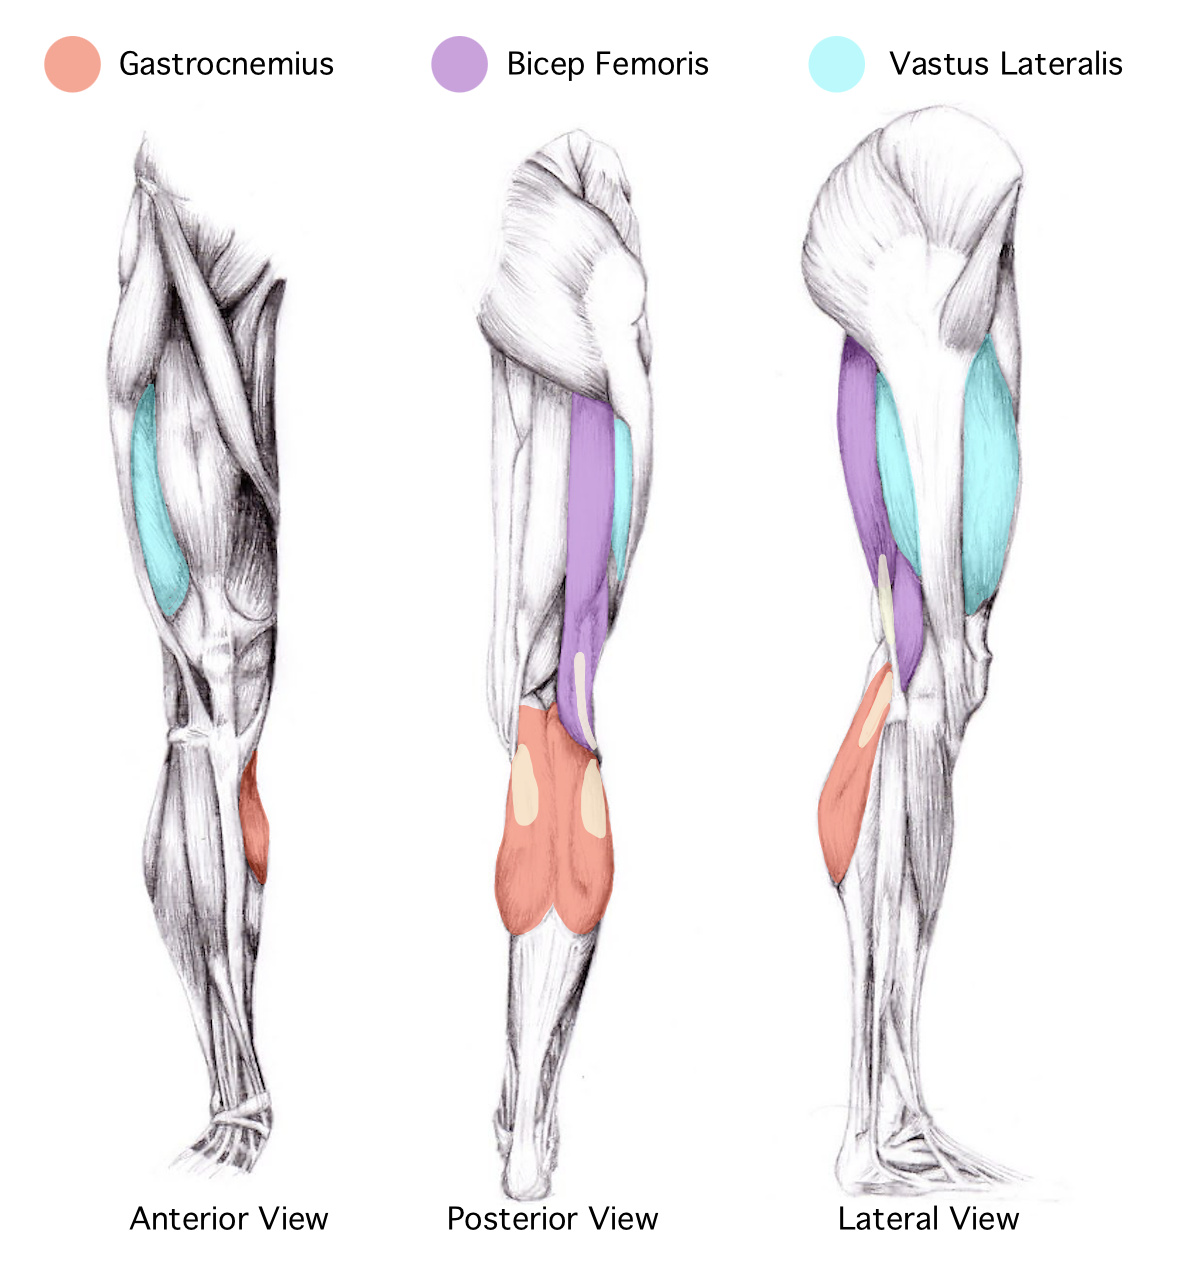
\includegraphics[scale=0.5]{Progress_Report/figs/highlightedmuscles.png}
\caption{Diagram of the Leg Muscles that will be Tested (highlighted are the muscles that will be tested)\cite{3}}
\label{fig:Muscles}
\end{figure}
\par


The Vastus Lateralis muscle is expected to have the greatest activity when the test subject is skating at a steady-state. The Gastrocnemius muscle is expected to have the greatest activity when the test subject is skating in order to increase their acceleration. The Bicep Femoris is expected to have the greatest activity when the test subject is skating at a steady-state.

\subsubsection{Progress}
For testing, the team has very limited amount of time on the ice per session so the team has developed a drill plan. These drills will be both the same for indoor roller skating and our on-ice hockey. For the testing the team will have five drills with varying intensity and varying muscles being targeting. These five drills will be our cross-over drill, stopping drill, laps around, forwards and backwards drill, and shooting. These drill can be observed in Figure 4.2.
\par
\begin{figure}[H]
\centering
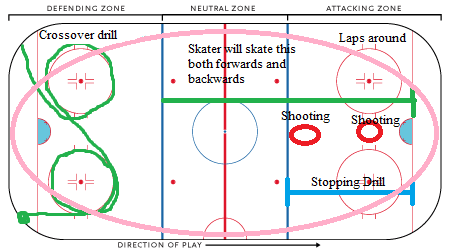
\includegraphics{Progress_Report/figs/HockeyRink-Zones.png}
\caption{Breakdown of the five drill participants will be demonstrating\cite{4}}
\label{fig:HockeyRink}
\end{figure}
\par
The cross-over drill is a high-intensity drill that involves the participant going around the circles located at the ends of the ice rink. This drill with have the participant go around the circle once then at continue on to the next circle going around it once. The next drill will then have the participant conducting the cross-over drill backwards. 

For the stopping drill, the participant will start at the goal line from rest and then accelerate to the blue line, where they will then stop. This drill is focused on the participant's force used in order to stop. 

The third drill will require the participant to skate laps around the rink. This is a lower intensity drill meant to focus on the EMG sensors that are placed on the test subject's legs, rather than the load sensors. The EMG sensors will be placed on the Vastus Lateralis, Gastrocnemius, and Bicep Femoris muscles. The low intensity drill will ensure that the activity of these three muscles can be accurately observed in steady-state skating, as well as accelerated skating. 

For the fourth drill, it will be the forwards and backwards drill. The participant will start at the goal line and then skate forwards to the far blue line before stopping and then skating backwards, this will show the participants muscles and load sensors when they stop and start back up when the participant starts skating backwards. This drill will give us a good reading on the muscles used to stop and start and going from forwards to backwards. 

The final drill will be our shooting drill, this drill will be from two different locations, on from the hash-marks, the other from the blue line. Each participant will get ten hockey pucks to shoot with. For these drills the placement of the EMG sensors will be changed to the lower back and arm muscles. The back and arm muscles that the EMG sensors will be placed on are the Latissimus Dorsi, Anterior Deltoid, and the Brachioradialis, displayed below in figure 4.3\cite{5}. The reference node for the EMG sensors on the back and arm will be placed on a spinous process.  
\par
\begin{figure}[htb]
\centering
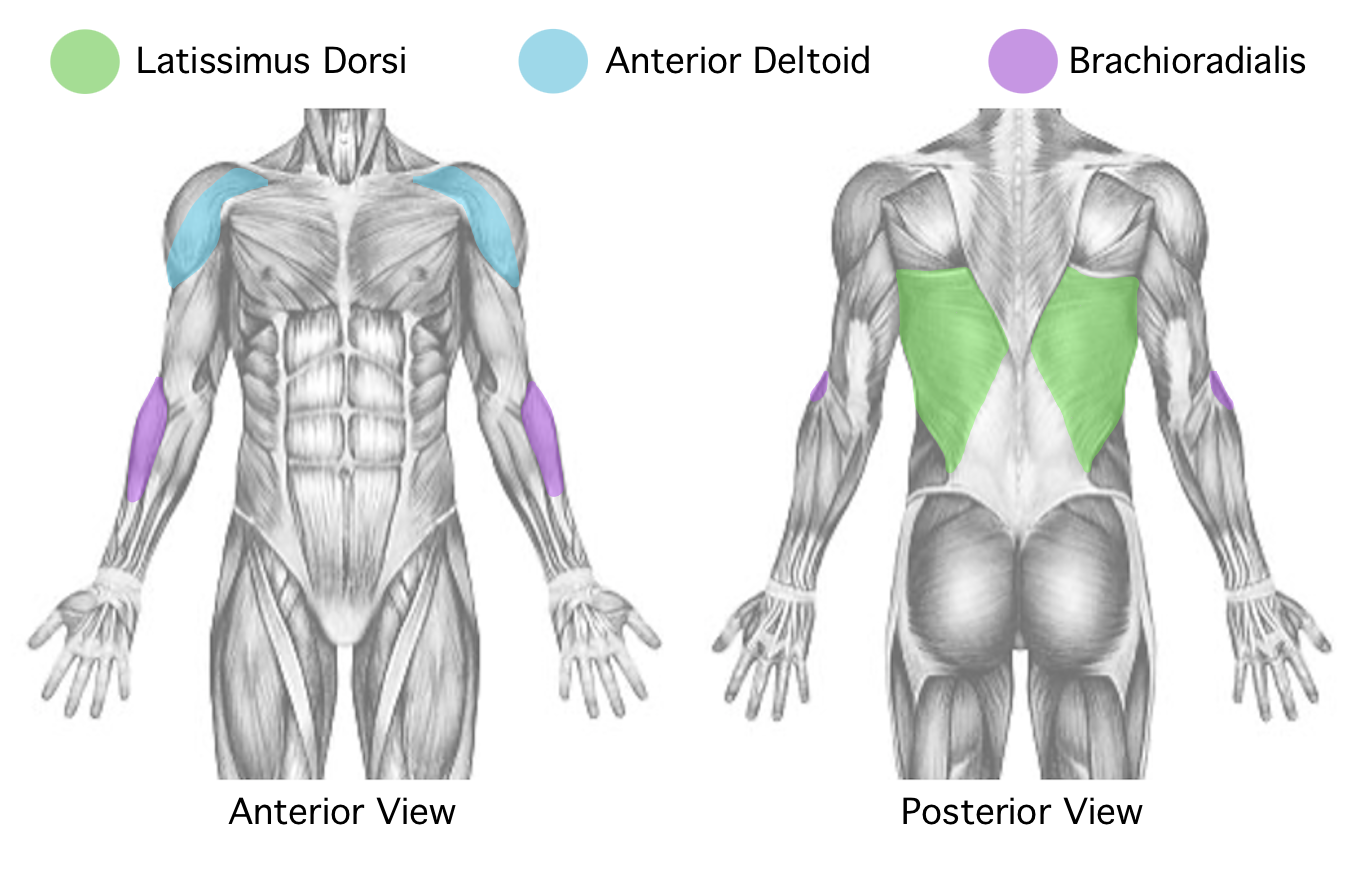
\includegraphics[scale=0.5]{Progress_Report/figs/shootingmuscles.png}
\caption{Diagram of the Back and Arm Muscles that will be Tested (highlighted are the muscles that will be tested)\cite{6}}
\label{fig:ShootingMuscles}
\end{figure}
\par
The Latissimus Dorsi muscle is a core muscle that is found on the lower back. The Latissimus Dorsi is an important muscle that contributed to the abduction, extension, and rotation of the arm\cite{5}. The Anterior Deltoid is a muscle that is found within the shoulder and contributes to the flexion of the arm and the rotation of the shoulder\cite{5}. The Anterior Deltoid is majorly used while in hockey for shooting and passing the puck\cite{7}. The Brachioradialis muscle is found in the forearm and is important in the bending and flexing of the elbow\cite{5}. The Brachioradialis is used in hockey for shooting the puck, as well as for control of the hockey stick\cite{7}.


%  6. Haredware Development

\subsection{Hardware Development}
\subsubsection{Variations from initial plans}
As mentioned in section 4.1.1, in order to have used the force sensitive resistors, the team would have had to make expand the circuitry on board with op-amps to permit readings greater than 20kg of force. At first this did not seem like a problem, but as the implementation went on the team realized this would introduce a large margin of error, and create for unreliable readings. For this reason the team made a switch to laod sensors which can measure up to 400kg when wired in series and can be calibrated to each skater giving. The team will have eight load sensors in total with four in each foot, offering 400kg of force to be collected from the skater, and providing for far more accurate results.
\subsubsection{Progress}
The team has made substantial development on the hardware, having completed the soldering of six EMG sensors into their required pins on the board and wires that will then connect to the arduino, as shown in the appendix. The arduinio has been programmed to send data to our ThingSpeak channel, where it will then be read by the software side of the project. The load cell sensors were all wired up in series, as there was four per series, the team had to solder eight load cell sensors in total as well as their amplifier module that needed the required pins to then be hooked up the arduino. This can be seen in the appendix 1.2. They have been finished and have been placed in soles of a shoe for easy access as the team will be switching participants frequently, and this will allow for a modular setup. The gyroscope is built into the board and has been setup to record the change of the boards position overtime.   


%  7. Software Development

\subsection{Software Development}
\subsubsection{Variations from initial plans}
During the sprint that will be discussed in further detail below, it was determined that Python and the Kivy framework were not a fully suitable technology stack for the needs of the team's application. The python library for visualization that the team investigated and used at the beginning of the sprint did not function well with real time updating of data, as well as requiring the environment to be properly set up on each local machine the application would be running on. There was also limited documentation and library options with that technology stack. Due to these limitations, as well as most of the software team having experience with building javascript web application, the decision was made, two days into the sprint to shift to building a web application using React framework for JavaScript where, through accessing a webpage on any device connected to the internet, it would be possible to access the GUI. Because of React's prevalence in the web development world, there is an abundance of documentation and libraries to help the the team develop the application that was initially envisioned and described in the Project Proposal. 

The role of the web application has also been expanded from original plans. Originally, the application was to serve as a method of monitoring real-time readings only, and all historical data was to be accessed through ThingSpeak. However, the team decided to congregate all data and functionality into one place - being the web application. This further allow the data to be organized the way the team decides is most useful for later data analysis, rather than it being dictated by ThingSpeak's structure. With the addition of the data history page, all data collected will be stored in the application's own database separate from ThingSpeak, and all data will be accessible from the data history page. With this expansion, a host of dropdowns and toggle switches that are set by the end user during operation and keep track of the type of drill, type of activity (skating or shooting), participant, and drill surface (ice or dryland) in order to organize as it passes from ThingSpeak to the application database through our application. 

A large architecture change was made since the project proposal. As outlined in section 9.2 of the Project Proposal, the architecture was to have a SQL database sitting between the Arduino board and the user application, allowing the application to fetch data from the database as the Arduino was uploading it. Allowing an Arduino to communicate data directly to a database, proved to be a very convoluted task that would involve using a rather undesirable method of communication: TCP/IP. The team promptly decided to switch to using ThingSpeak, a MathWorks product, made exactly for this purpose, to facilitate communication between the Arduino and the application. The database would still be involved in the architecture, standing behind the application, allowing all the data that comes through the application from ThingSpeak, to be stored in a database carefully configured by the team. Considering the tech stack for the application changed substantially, it was logical to change the database to a nosql cloud-based database provided by Google Firebase, as it provided easier connection and data manipulation through the current tech stack. The new architecture can be seen in the following section
\begin{figure}[H]
\centering
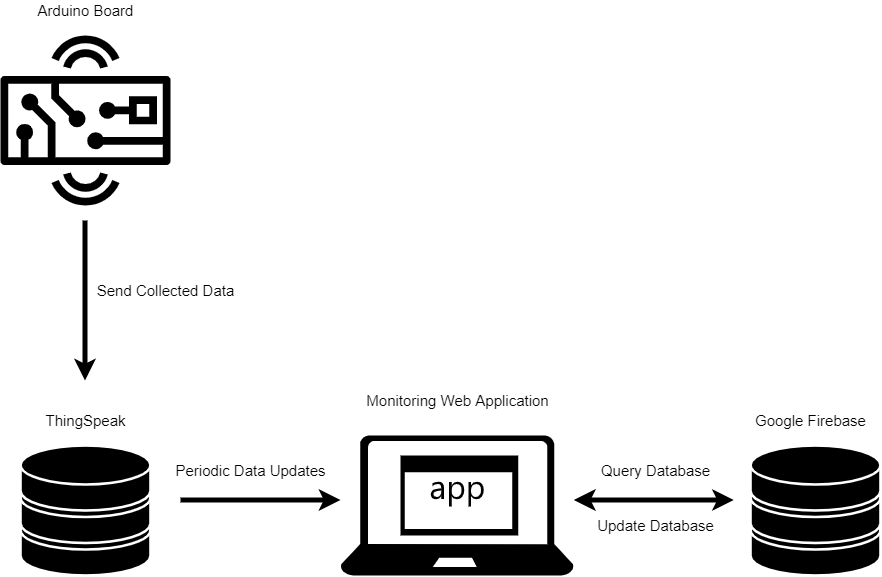
\includegraphics[width =\textwidth]{Progress_Report/figs/CapstoneDiagrams-Page-2.drawio (1).png}
\caption{Remodelled software process}
\label{fig:ThingSpeak}
\end{figure}
\par
\subsubsection{Progress}
In the new year, the software team organized a sprint spanning the last nine days of the winter break. The sprint saw the beginning and large progress in the development of the Data Collection and Monitoring Web Application and its data component. 

The team's progressed by connecting the data middleman (between hardware and software), ThingSpeak, to the front end. Being able to have multiple channels with each have multiple fields has been very helpful for the team. Each type of sensor has been assigned it's own channel, with each sensor within the three types being assigned its own field. For example, the EMG sensors have their own channel, with each of the 6 EMG sensors representing one field in that channel. 

\begin{figure}[htbp]
\centering
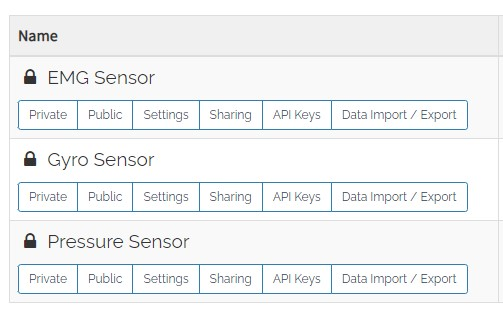
\includegraphics[scale=0.9]{Progress_Report/figs/ThingspeakChannels.jpg}
\caption{Demonstration of the breakdown of Thingspeak}
\label{fig:ThingSpeak1}
\end{figure}

\begin{figure}[H]
\centering
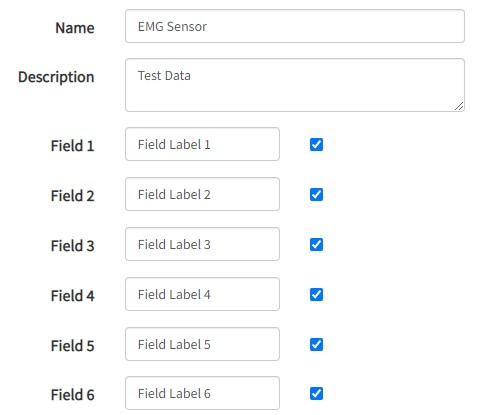
\includegraphics[scale=0.9]{Progress_Report/figs/ThingspeakFields.jpg}
\caption{Demonstration of the breakdown of Thingspeak}
\label{fig:ThingSpeak2}
\end{figure}

Since the Arduinos that control the sensors will be sending data every one second to their respective channels and fields, the application will be fetching this data every one second as well. Doing so will allow for timely collection and visualization. In addition, the team was able to use JavaScript's synchronous nature to their advantage. In doing so, the team was able to avoid the needing to create a multithreaded web application. The part of the code that fetches the data from ThingSpeak will be executed one channel at a time. This is executed so quickly that it is virtually indistinguishable from a concurrent set of fetches on the front end side, and will display every single data point from every single sensor at the same time on a one-second interval. 

\paragraph{Data Collection and Monitoring Web App}


The web application's graphical user interface was wire framed, and subsequently built out. The design of the web application would consist of 5 total pages: An overview page where current real-time readings of each sensor can be seen all at once, 1 page for each of the 3 sensor types, that will show a readings table and graph visualizing the readings as they come in. There is also a data history page that will allow the end user to browse all data collected.

The data collection web application is built using a stack consisting of ReactJS and NodeJS Frameworks. The application was built with a component-based approach, where the construction began by building the components that would be found on the pages of the application. To date, the gauge component that will be displayed on the overview dashboard to display the reading on the host of sensors concurrently collecting data was built. The data table components that will dynamically display incoming readings from individual sensors on their respective pages were built. Also built was the graph component that will graphically and dynamically display individual sensor readings on their respective pages. The team has built out the common frame of the web application consisting of the navigation bar, and filtering options consisting of drop-down, and toggle switches which will allow the end user to input the parameters of the data currently being observed. 

\begin{figure}[h]
     \centering
     \begin{subfigure}[h]{0.45\textwidth}
         \centering
         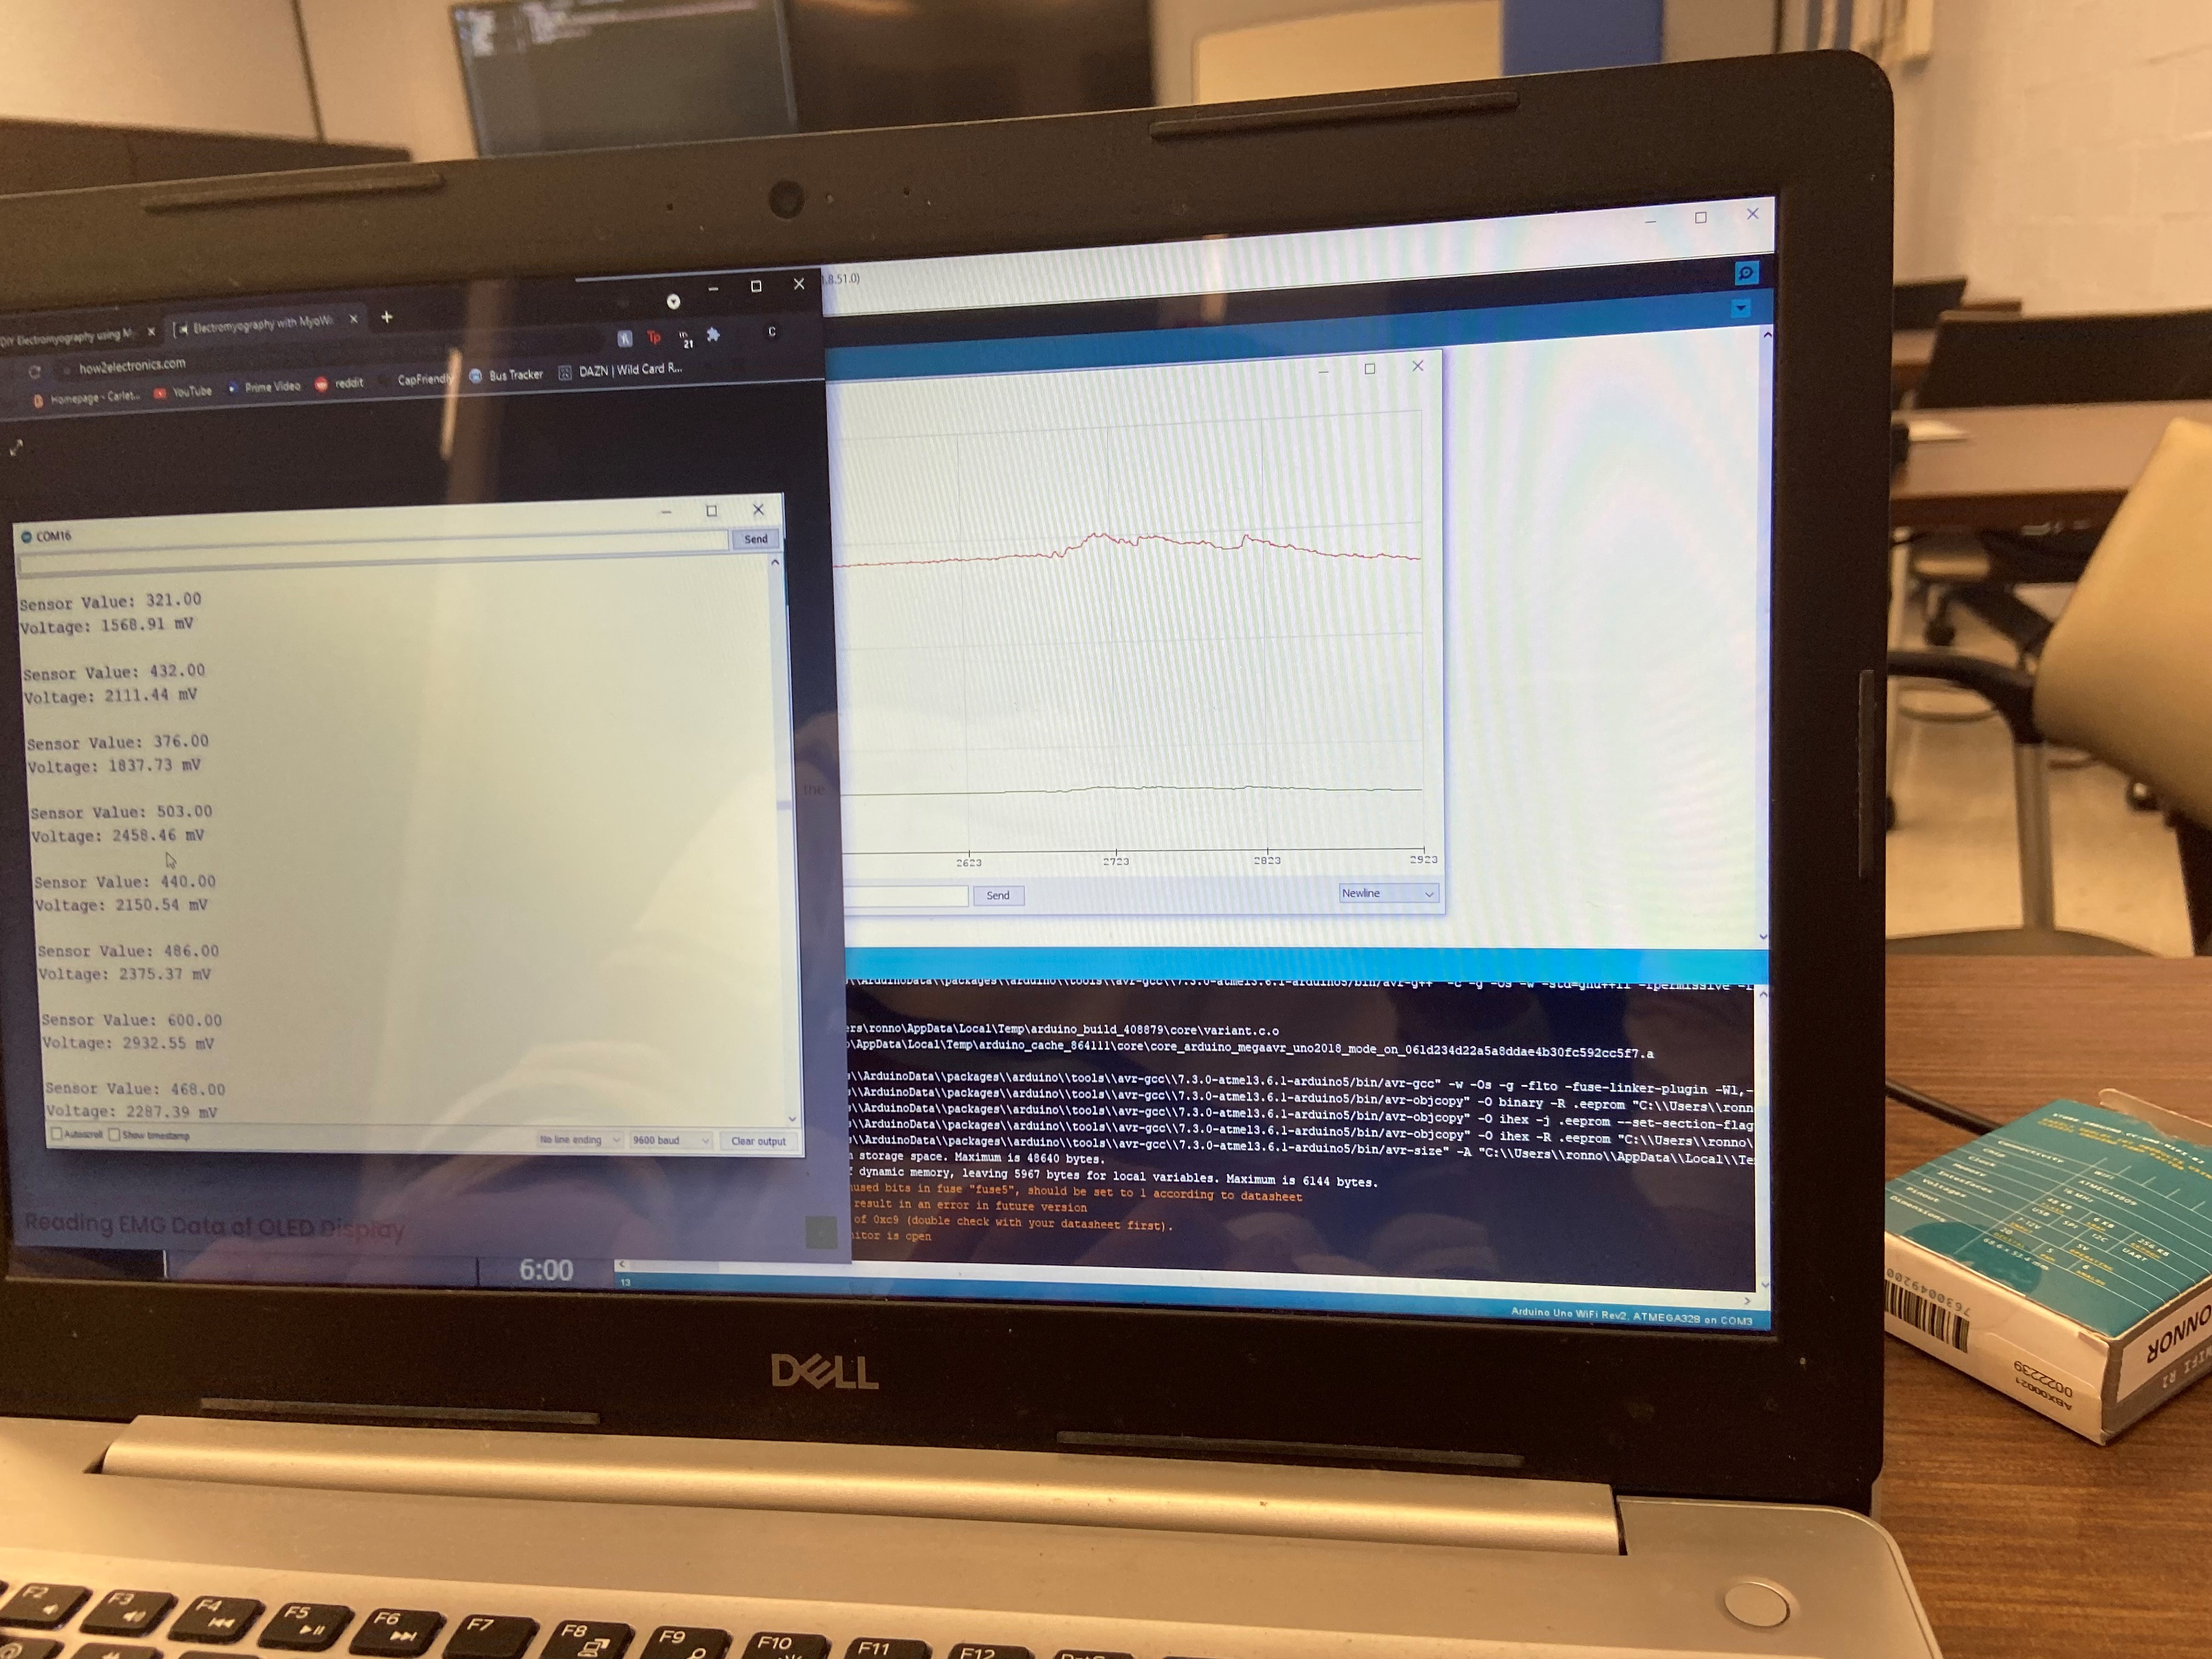
\includegraphics[width=\textwidth]{Progress_Report/figs/EmgReadings.jpg}
         \caption{List of data that was gathered}
         \label{fig:EMG Readings}
     \end{subfigure}
     \hfill
     \begin{subfigure}[h]{0.45\textwidth}
         \centering
         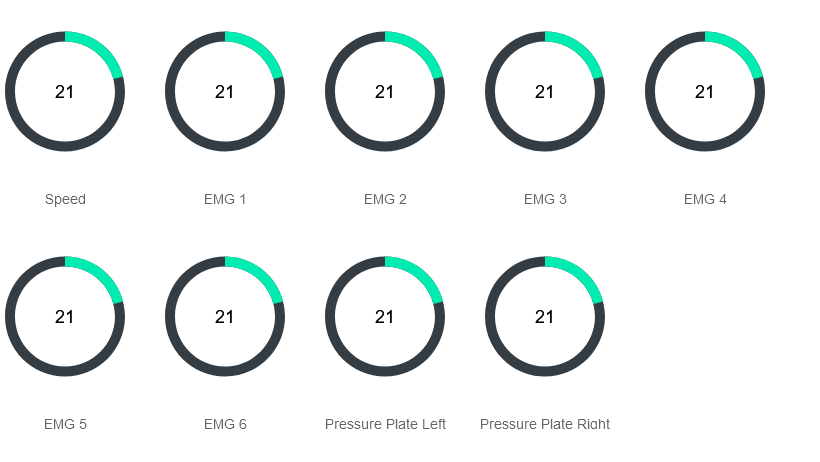
\includegraphics[width=\textwidth]{Progress_Report/figs/emgs.png}
         \caption{Gauges for real time viewing}
         \label{fig:emg gauges}
     \end{subfigure}
     \hfill
     \begin{subfigure}[h]{0.45\textwidth}
         \centering
         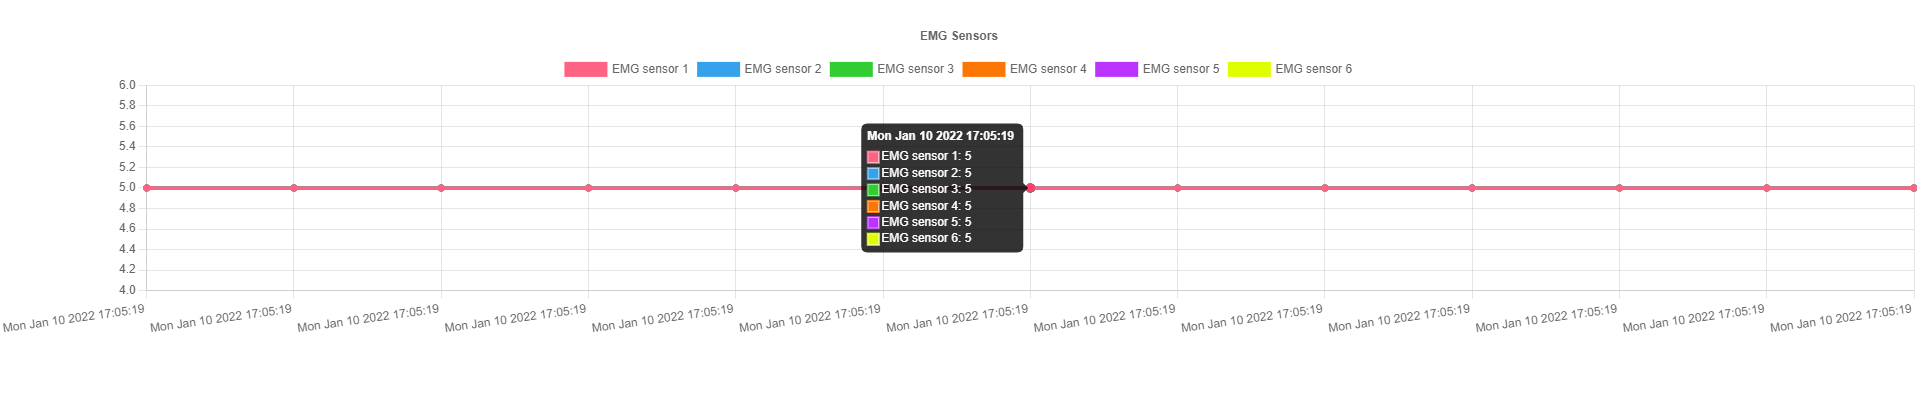
\includegraphics[width=\textwidth]{Progress_Report/figs/graph.png}
         \caption{graph showing data gathered from the EMG sensors.}
         \label{fig:graph}
     \end{subfigure}
     \begin{subfigure}[h]{0.45\textwidth}
         \centering
         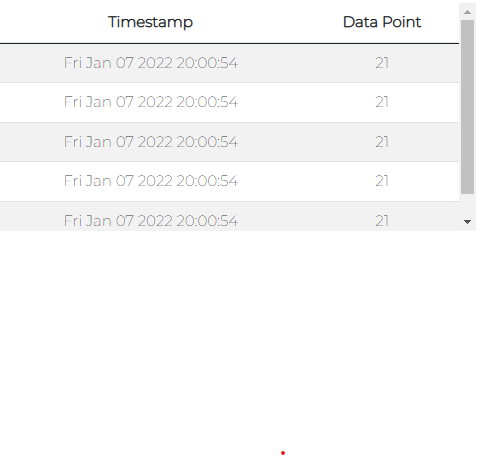
\includegraphics[width=\textwidth]{Progress_Report/figs/data_table.png}
         \caption{Data Table}
         \label{fig:table}
     \end{subfigure}
     \begin{subfigure}[h]{\textwidth}
         \centering
         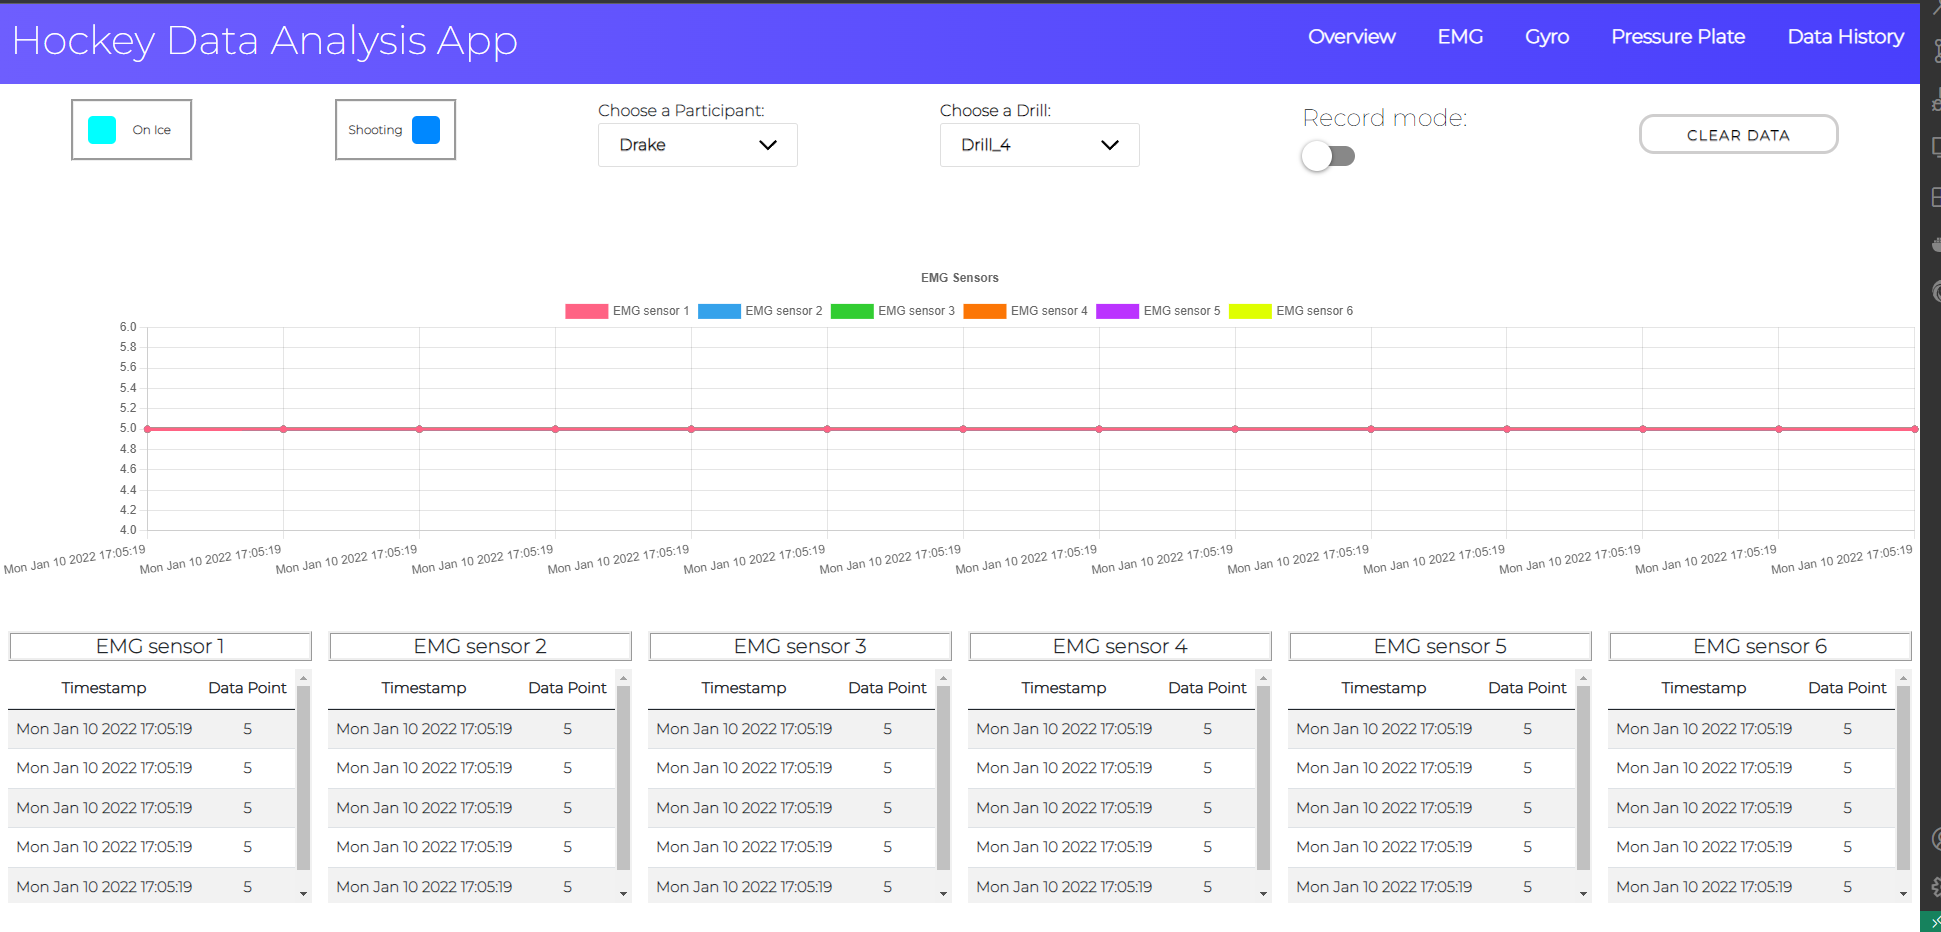
\includegraphics[width=\textwidth]{Progress_Report/figs/graph_table.png}
         \caption{Example of one of the individual sensor pages displaying its graph and individual sensor tables}
         \label{fig:table}
     \end{subfigure}     
     
        \caption{Software output}
        \label{fig:three graphs}
\end{figure}





%  8. Next Steps

\section{Next Steps}

The team will continue working on the development of the Data Collection and Monitoring Web App. The next steps for the application consist of assembling all the individual pages, and developing the functionality that will permit data to be stored on the data history page. The team will also work on formatting and connecting a database to store all historical data. Once those steps are complete, the application should be fully functional for testing and data collection. 

The next steps on the hardware side are to get all the sensors working concurrently and transmitting data to ThingSpeak. Once all sensors are working concurrently, the system will be configured for wearability for the test participants and ready for testing.   

Due to the current circumstances surrounding COVID-19 lockdowns in the region, the team has prepared a contingency plan. Since it is winter the team will shift to using outdoor public skating rinks. This will introduce challenges as the ice quality will be severely reduced on outdoor rinks, and whether conditions can be a large factor that may affect the ability to collect data and the quality of data being collected. When using the outdoor rinks there will not be previously existing markers that are on an indoor ice rink. In order to perfectly mimic these marks for the outdoor rinks, the team will be using markers and pylons in order to effectively execute the planned testing drills. For the dry-land aspect of the data gathering, the team will be attempting to utilize snow-cleared parking lots. Again, these conditions are not ideal, however due to the circumstances and budgetary constraints of the team, it is the most reasonable backup option. Of course, if the lockdown is no longer active by the time the team reaches the data gathering steps then they will continue on with their original plans and conduct the proceeding experiments inside, when possible. 


%  9. Updated Roles

\newpage
\section{Roles}
%have caption aboe the table
\begin{table}[ht]
\begin{center}
\begin{tabular}{|m{3cm}|m{2cm}|m{22em}|}
\hline
Member & Team & Involvement \\ 
\hline
\hline
Braden Hayes & Software & Software Design and Requirements Elicitation and Planning, Sprint Planning, Web Application Development \\ 
\hline
Mario   Shebib & Software & Software Design and 
Requirements Elicitation and Planning, Sprint Planning, Web Application Development \\ 
\hline
Marko   Majkic & Software & Software Design and Requirements Elicitation and Planning, Sprint Planning, Web Application Development \\ 
\hline
Drake Mcgillivray & Hardware  & Hardware Design and Construction (Pressure Sensors and EMG Sensors), Software (Connecting hardware to software)\\ 
\hline
Kate   Delaney & Hardware & Activity of Muscles, Hardware Design and Construction (EMG Sensors), Visualization of Data, Analysis of Data (MATLAB)\\ 
\hline
Connor Judd & Hardware & Hardware Design and Construction (Arduino Coding and Implementation, Circuit construction )\\ 
\hline

\end{tabular}
\caption{Proposed Alternative format for roles listing}
\label{table:roles}
\end{center}
\end{table}

%  10. Conclusion

\section{Conclusion}
The project continues to proceed on schedule with minor interruptions due to the COVID-19 pandemic. The hardware portion of the project is near completion. The prototype is designed and will merely need to be put together, and will then be ready for implementation. Additionally, the software portion of the project is near completion. The Data Collection and Monitoring Web Application was designed and continues to be developed on schedule. A data history page on the app needs to be developed and the software will then be ready to be connected to the hardware. It is expected that the testing and collection of the data will be completed by mid-February with dependencies on the possible inclement weather. The project team continues to work as a collaboratively in their respective sub-teams, and a whole, and is determined to stay on schedule and meet all of the internal deadlines that were specified.

%  11. Appendix References

\end{flushleft}
\begin{landscape}

\section*{Appendix}
%make it more readable gantt chart.
\begin{figure}[htbp]
\centering
\includegraphics[scale=0.25]{Final_Report/figs/FinalreportGantt-Page-1.drawio(1).png}
\caption{A Gantt Chart visualization of the in-completed timetable that will be finished for submission \ref{table:1}}
\label{fig:Appendix}
\end{figure}
\end{landscape}
\begin{figure}[htbp]
\centering
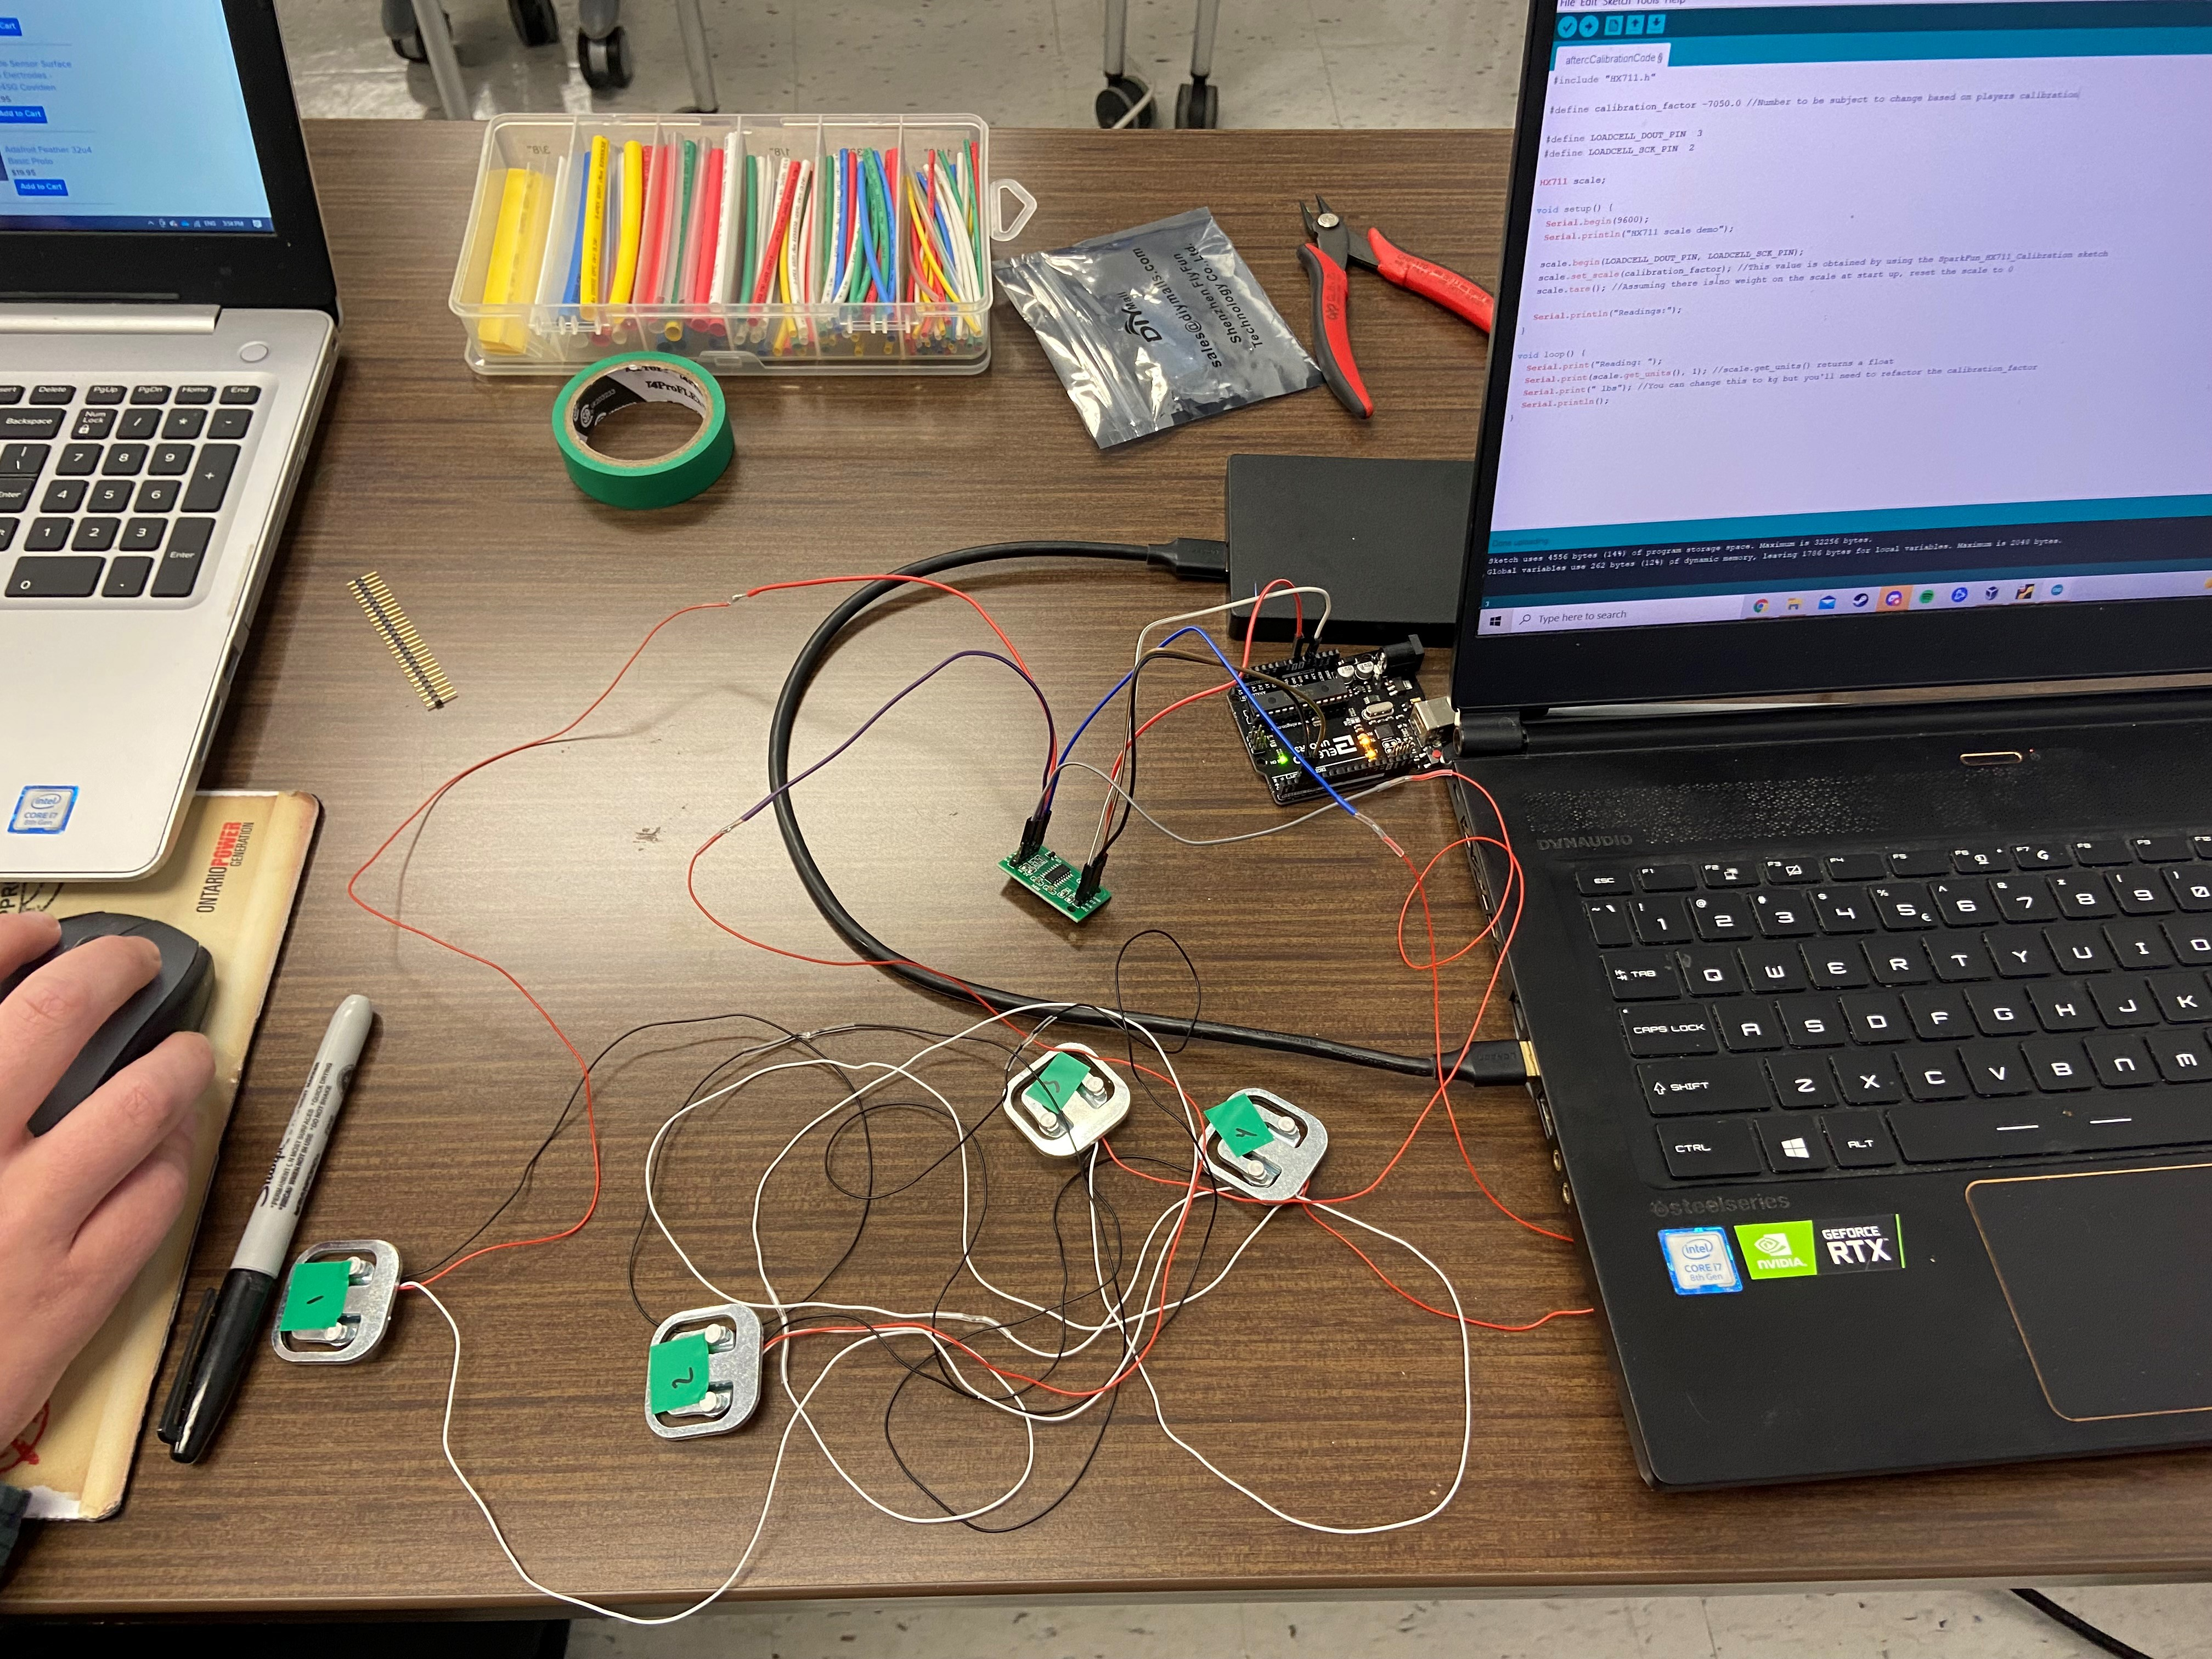
\includegraphics[scale=0.1]{Final_Report/figs/Loadcell_sensors.jpg}
\caption{Load cell sensors being tested after being wired in series}
\label{fig:loadcell}
\end{figure}
\begin{figure}[htbp]
\centering
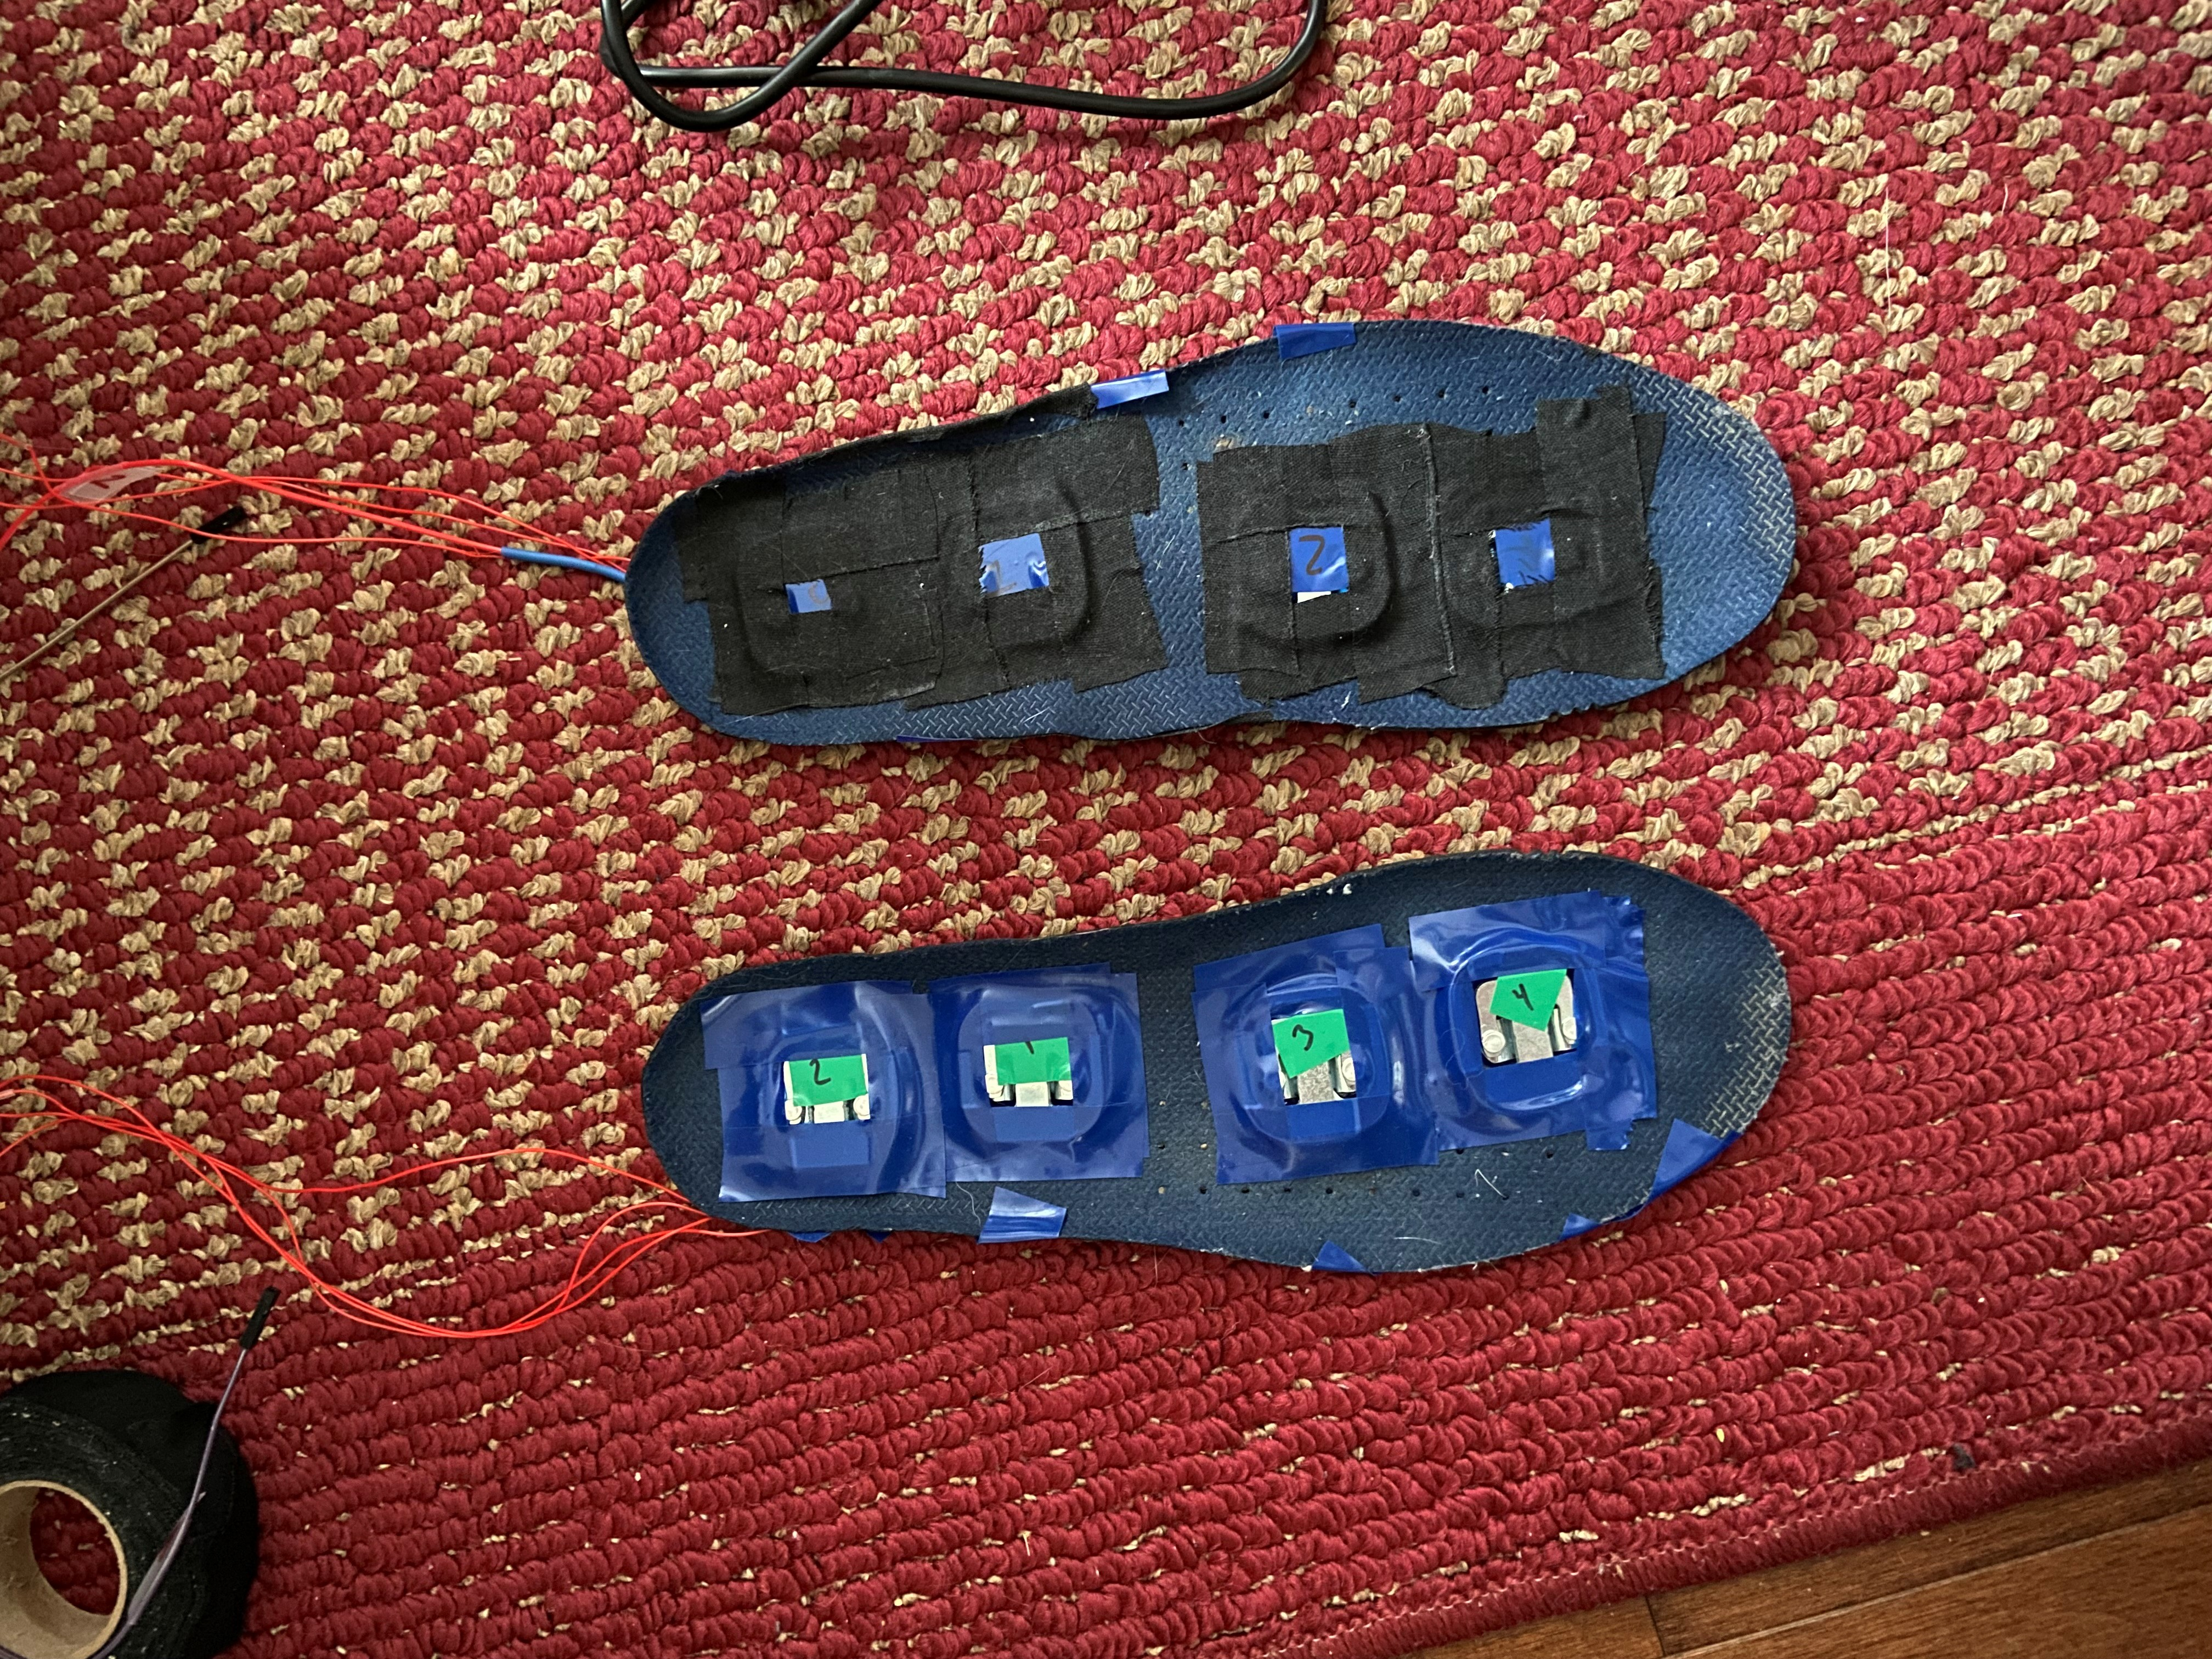
\includegraphics[scale=0.1]{Final_Report/figs/Loadcell_sensors_sole.jpg}
\caption{Load cell sensors place in the insoles prepared for testing}
\label{fig:loadcell}
\end{figure}
\begin{figure}[htbp]
\centering
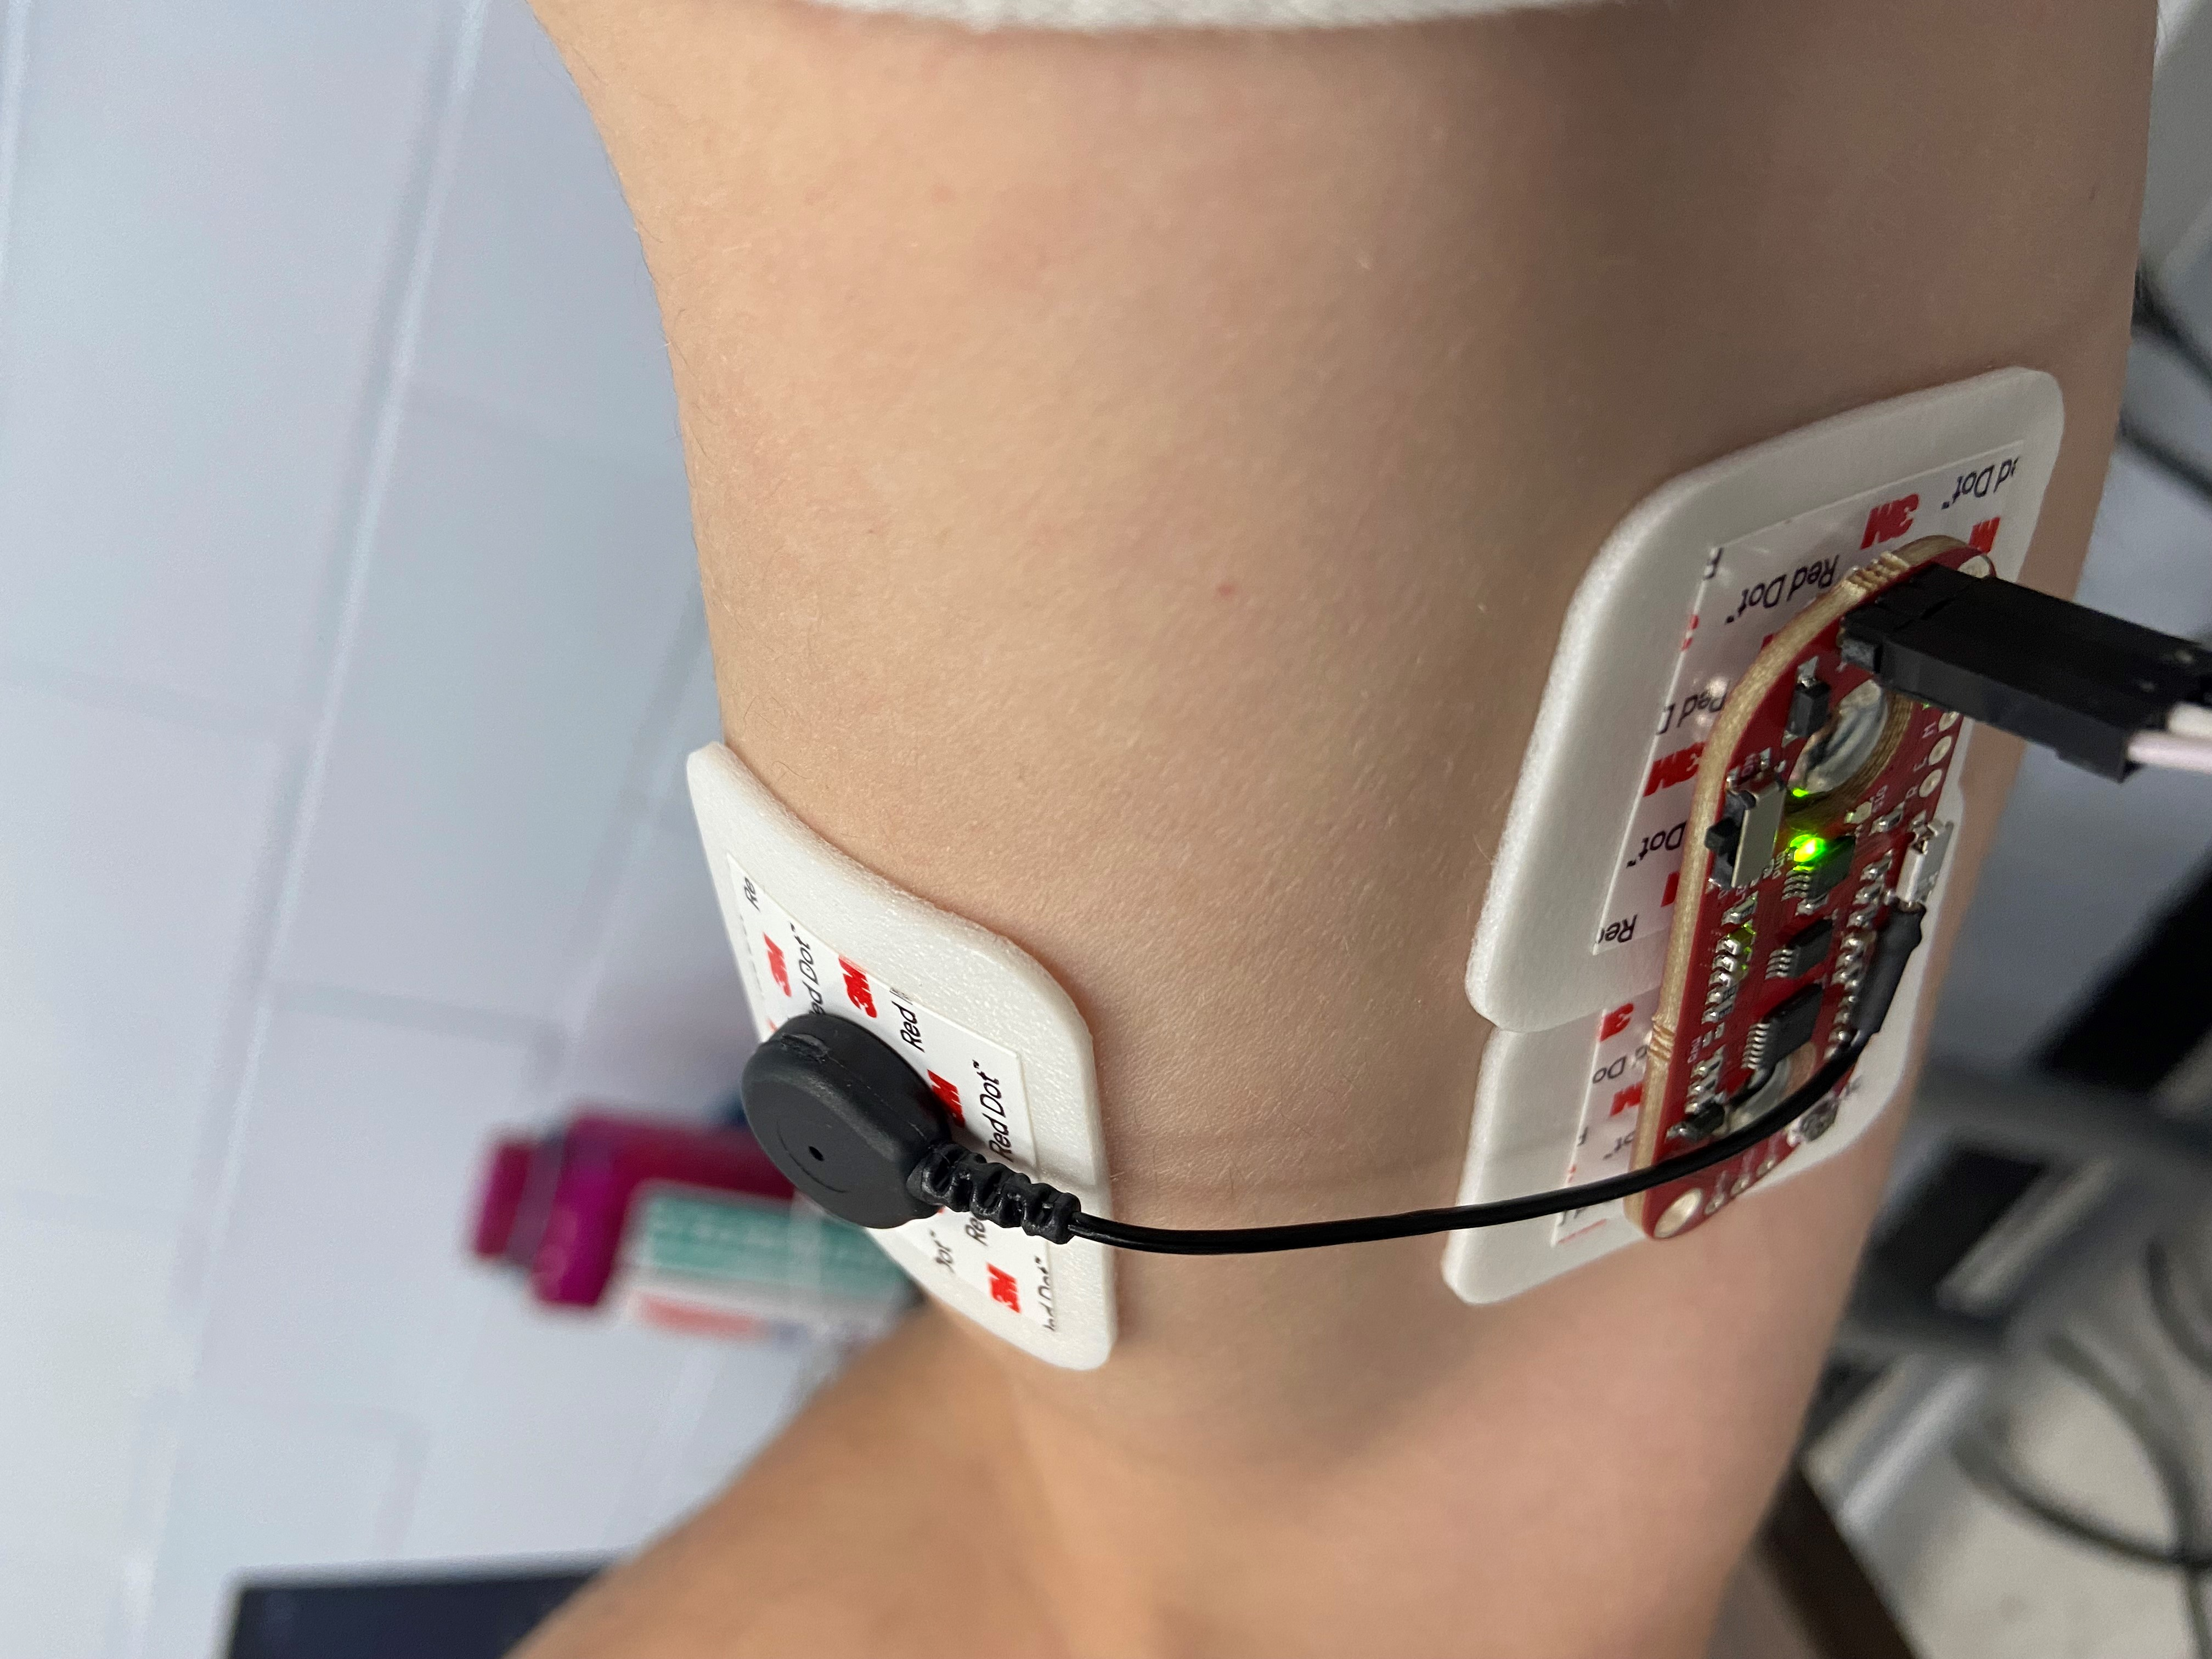
\includegraphics[scale=0.1]{Final_Report/figs/SensorPlacement.jpg}
\caption{Testing muscle placement to get proper readings} %Include what type of hardware are being used
\label{fig:sensorplacement}
\end{figure}
\newpage
\subsection*{Project Proposal}
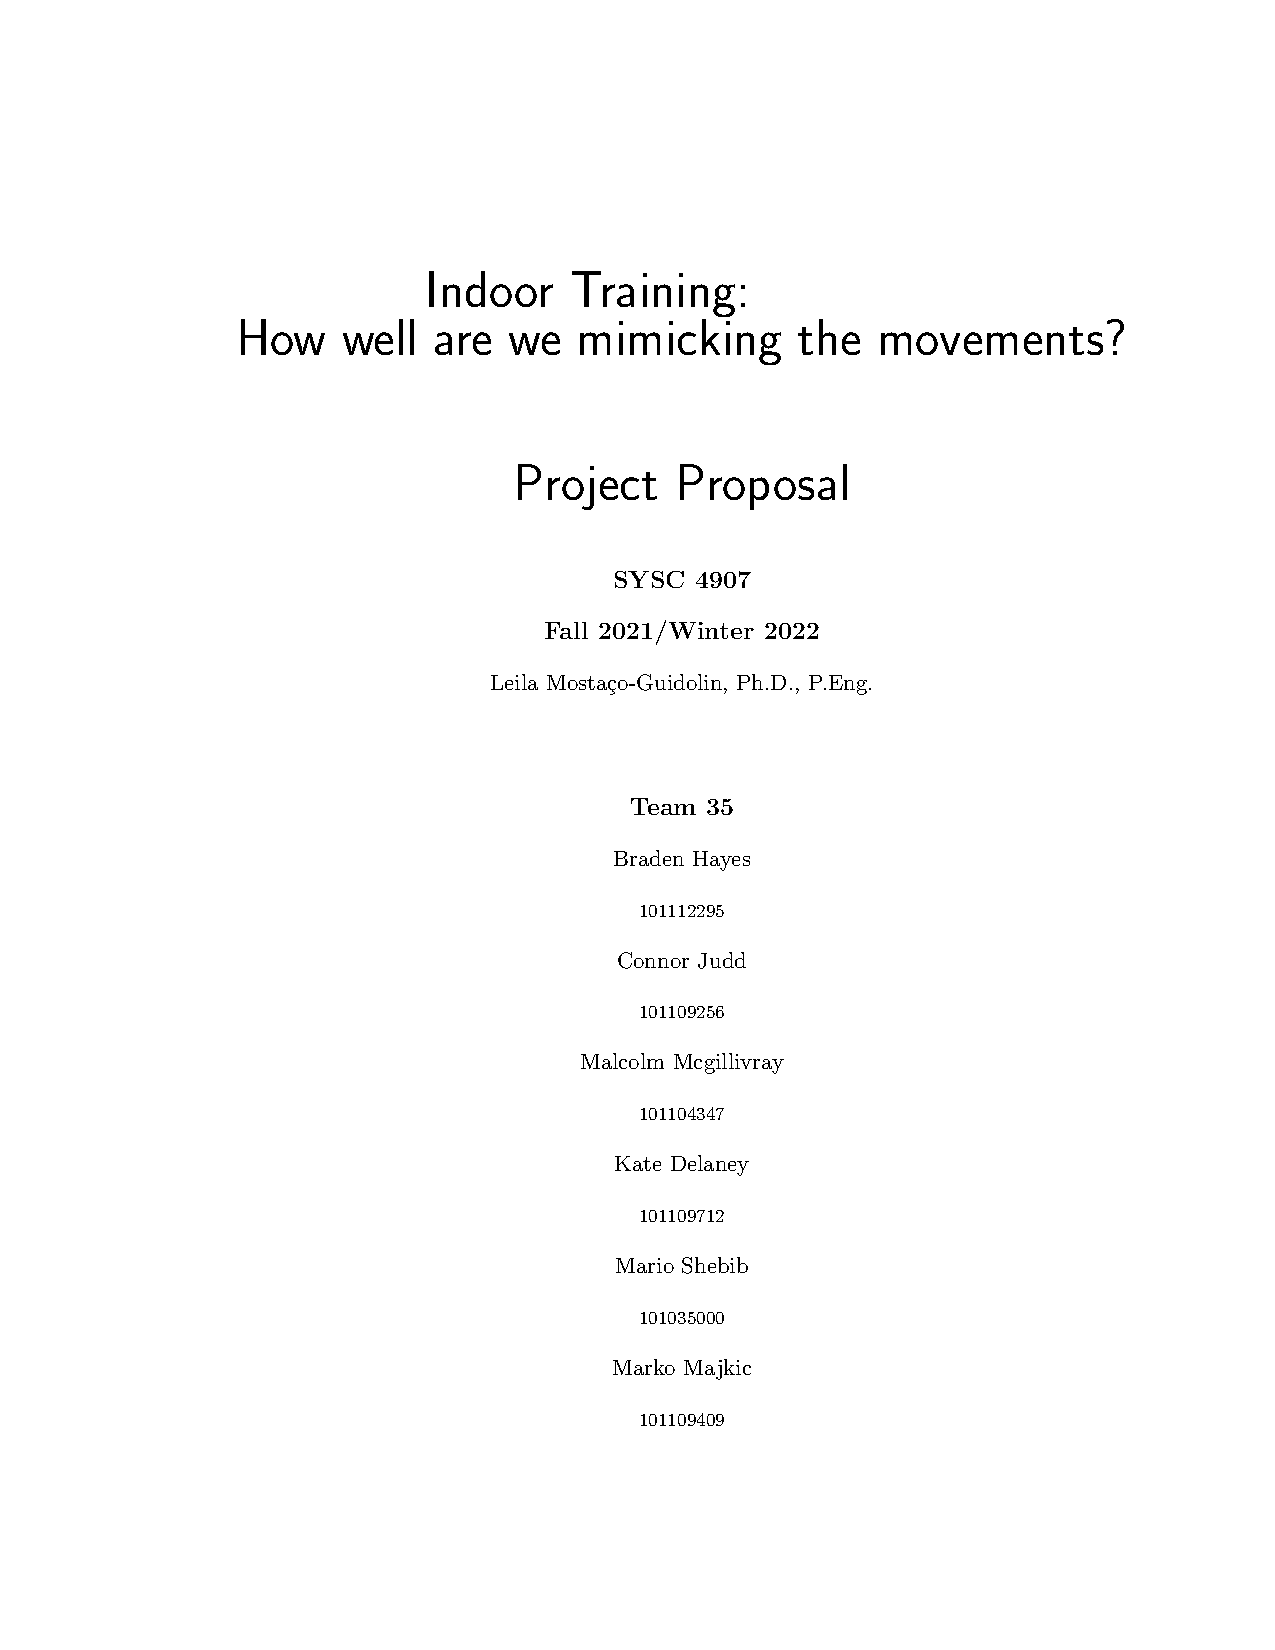
\includepdf[pages=-,pagecommand=\thispagestyle{plain}]{pdfs/Project_Proposal.pdf}
%make sure it's IEEE standard format
\bibliographystyle{IEEEtran}
\bibliography{Final_Report/refs}
\end{document}
